%%=============================================================================
%% Loki
%%=============================================================================

\chapter{Loki}
\label{ch:loki}

\section{Installatie en configuratie}

\subsection{Lokale omgeving}
De lokale installatie van de Loki stack kan volledig overgenomen worden van de officiële documentatie van Loki die te vinden is op github.com/grafana/loki. Er zijn 3 belangrijke stappen bij installeren van deze stack. 
\begin{enumerate}
    \item Promtail zoekt de log files in de locaties die gespecifieerd worden in de configuratie (zie listing 7.1). Daarna stuurt deze ze door naar Loki waar ze opgeslagen worden.
    \item Loki slaat de logs die via de gespecifieerde poort binnenkomen via Promtail.
    \item Grafana is de frontend van deze stack, hier worden de eerste 1000 logs van Loki binnengehaald en overzichtelijk gepresenteerd.
\end{enumerate}

Grafana biedt ook een gratis cloud hosted oplossing aan voor test doeleinden. Indien gebruik gemaakt wordt van deze oplossing moet enkel promtail geconfigureerd worden. Documentatie hiervoor is te vinden op de documentatie pagina van Grafana.

\subsubsection{Promtail}
De belangrijkste configuratie punten van de configuratie in Listing 7.1 worden hier besproken.

Een eerste belangrijk configuratie punt is de client url. Deze definieert waar de gevonden logs naartoe worden gestuurd. Bij de lokale configuratie zal dit altijd localhost zijn. De poort 3100 die in Listing 7.1 gedefineerd staat, is terug te vinden in Listing 7.2 als de poort van Loki waarop geluisterd wordt naar binnenkomende calls.

Een tweede belangrijk configuratie punt is de scrapeconfigs. Deze definieert alles van het scrapen logs. In zijn simpelste vorm, zoals te zien is in Listing 7.1, gaat het slechts om 1 job die op zoek gaat naar logs in slechts 1 locatie. Deze configuratie kan snel ingewikkeld worden wanneer sprake is van meerdere jobs die elk meerdere locaties in de gaten houden. Elke locatie heeft zijn eigen label. Zo worden de logs in Grafana makkelijker gefilterd en zullen deze overzichtelijker te tonen zijn. Een andere manier om de configuratie ingewikkelder te maken is het blacklisten van sommige locaties. Dit wil zeggen dat sommige locaties genegeerd worden terwijl andere wel gescrapet worden. Extra informatie over de volledige configuratiemogelijkheden zijn te vinden op github.com/grafana/loki.

Deze configuratie wordt op zijn beurt gebruikt binnen docker container die te vinden is in de officiële docker hub repositories van Grafana, namelijk hub.docker.com/u/grafana. Bij het aanmaken van deze container moet ook een volume gespecifieerd worden. Dit volume is een locatie in de lokale omgeving die gekoppeld wordt met de container. Het commando in dit voorbeeld is te zien op Listing 7.2.

\begin{lstlisting}[caption=promtail-config yaml file ]
server:
    http_listen_port: 9080
    grpc_listen_port: 0

positions:
    filename: /tmp/positions.yaml

client:
    url: http://localhost:3100/api/prom/push

scrape_configs:
    - job_name: log-test
        entry_parser: raw
        static_configs:
        - targets:
            - localhost
        labels:
            job: bp
            __path__: /etc/promtail/logs/*.log  
\end{lstlisting}

\begin{lstlisting}[caption=Aanmaken van de promtail container]
$ docker run --name promtail --volume "$PWD:/etc/promtail" grafana/promtail:master -config.file=/etc/promtail/config.yaml
\end{lstlisting}

\subsubsection{Loki}

De belangrijkste configuratie punten van de configuratie in Listing 7.3 worden hier besproken.

Een eerste belangrijk configuratiepunt is de http listen port. Zoals reeds vermeld in de subsectie Promtail hierboven is dit de poort waar Loki naar luistert en Promtail logs naar stuurt. 

Een tweede belangrijk configuratiepunt is de ingester. De functie hiervan werd reeds besproken in de literatuurstudie van dit werk. 

Een derde belangrijk configuratiepunt is de schema config. Deze definieert de databanken waar de chunks en indexen opgeslagen worden. De chunks worden in een objectstore opgeslagen. In een basis lokale configuratie zal dit het filesystem zijn zoals in Listing 7.3 maar er zijn reeds andere object store databanken ondersteund door Grafana. Voorbeelden hiervan zijn Google Cloud en AWS S3. De indexen worden opgeslagen in een NoSQL databank. Standaard staat deze ingesteld op boltdb, wat een lokale NoSQL databank is. Ook deze databank kan veranderd worden door een gewenste databank.

Een laatste belangrijk punt in de configuratie van Loki is de storage config. Zoals hierboven reeds vermeld worden de indexen en chunks opgeslagen in respectievelijk een NoSQL databank en een Object Store. De locatie hiervan wordt in deze configuratie gespecifieerd.

Deze configuratie wordt op zijn beurt gebruikt binnen docker container die te vinden is in de officiële docker hub repositories van Grafana, namelijk hub.docker.com/u/grafana. Het commando in dit voorbeeld is te zien op Listing 7.2.

\begin{lstlisting}[caption=Loki config yaml file]
auth_enabled: false

server:
    http_listen_port: 3100

ingester:
    lifecycler:
        address: 127.0.0.1
        ring:
            store: inmemory
            replication_factor: 1
        chunk_idle_period: 15m

schema_config:
    configs:
        - from: 0
            store: boltdb
            object_store: filesystem
            schema: v9
            index:
                prefix: index_
                period: 168h

storage_config:
    boltdb:
        directory: /tmp/loki/index

    filesystem:
        directory: /tmp/loki/chunks

limits_config:
    enforce_metric_name: false
\end{lstlisting}

\begin{lstlisting}[caption=Aanmaken van Loki container]
$ docker run --name loki grafana/loki:latest -config.file=/etc/loki/local-config.yaml
\end{lstlisting}

\subsubsection{Grafana}

Om Grafana lokaal te hosten wordt gebruik gemaakt van Homebrew voor Mac OS. Met twee simpele commando's, Listing 7.5 en Listing 7.6 wordt Grafana opgestart op de standaard poort, namelijk 3000.

De volgende stap is Loki linken met Grafana. Dit gebeurt door Loki als datasource te selecteren in de Grafana UI. Daarna zijn de logs te zien in het Explore tab van de UI. Nu is het mogelijk om logs te filteren en te queriën op label of job zoals te zien is in Afbeelding 7.1.

\begin{lstlisting}[language=bash, caption=install grafana]
$ brew install grafana
\end{lstlisting}
\begin{lstlisting}[language=bash, caption=start grafana]
$ brew services start grafana
\end{lstlisting}

\begin{figure}[ht]
    \centering
    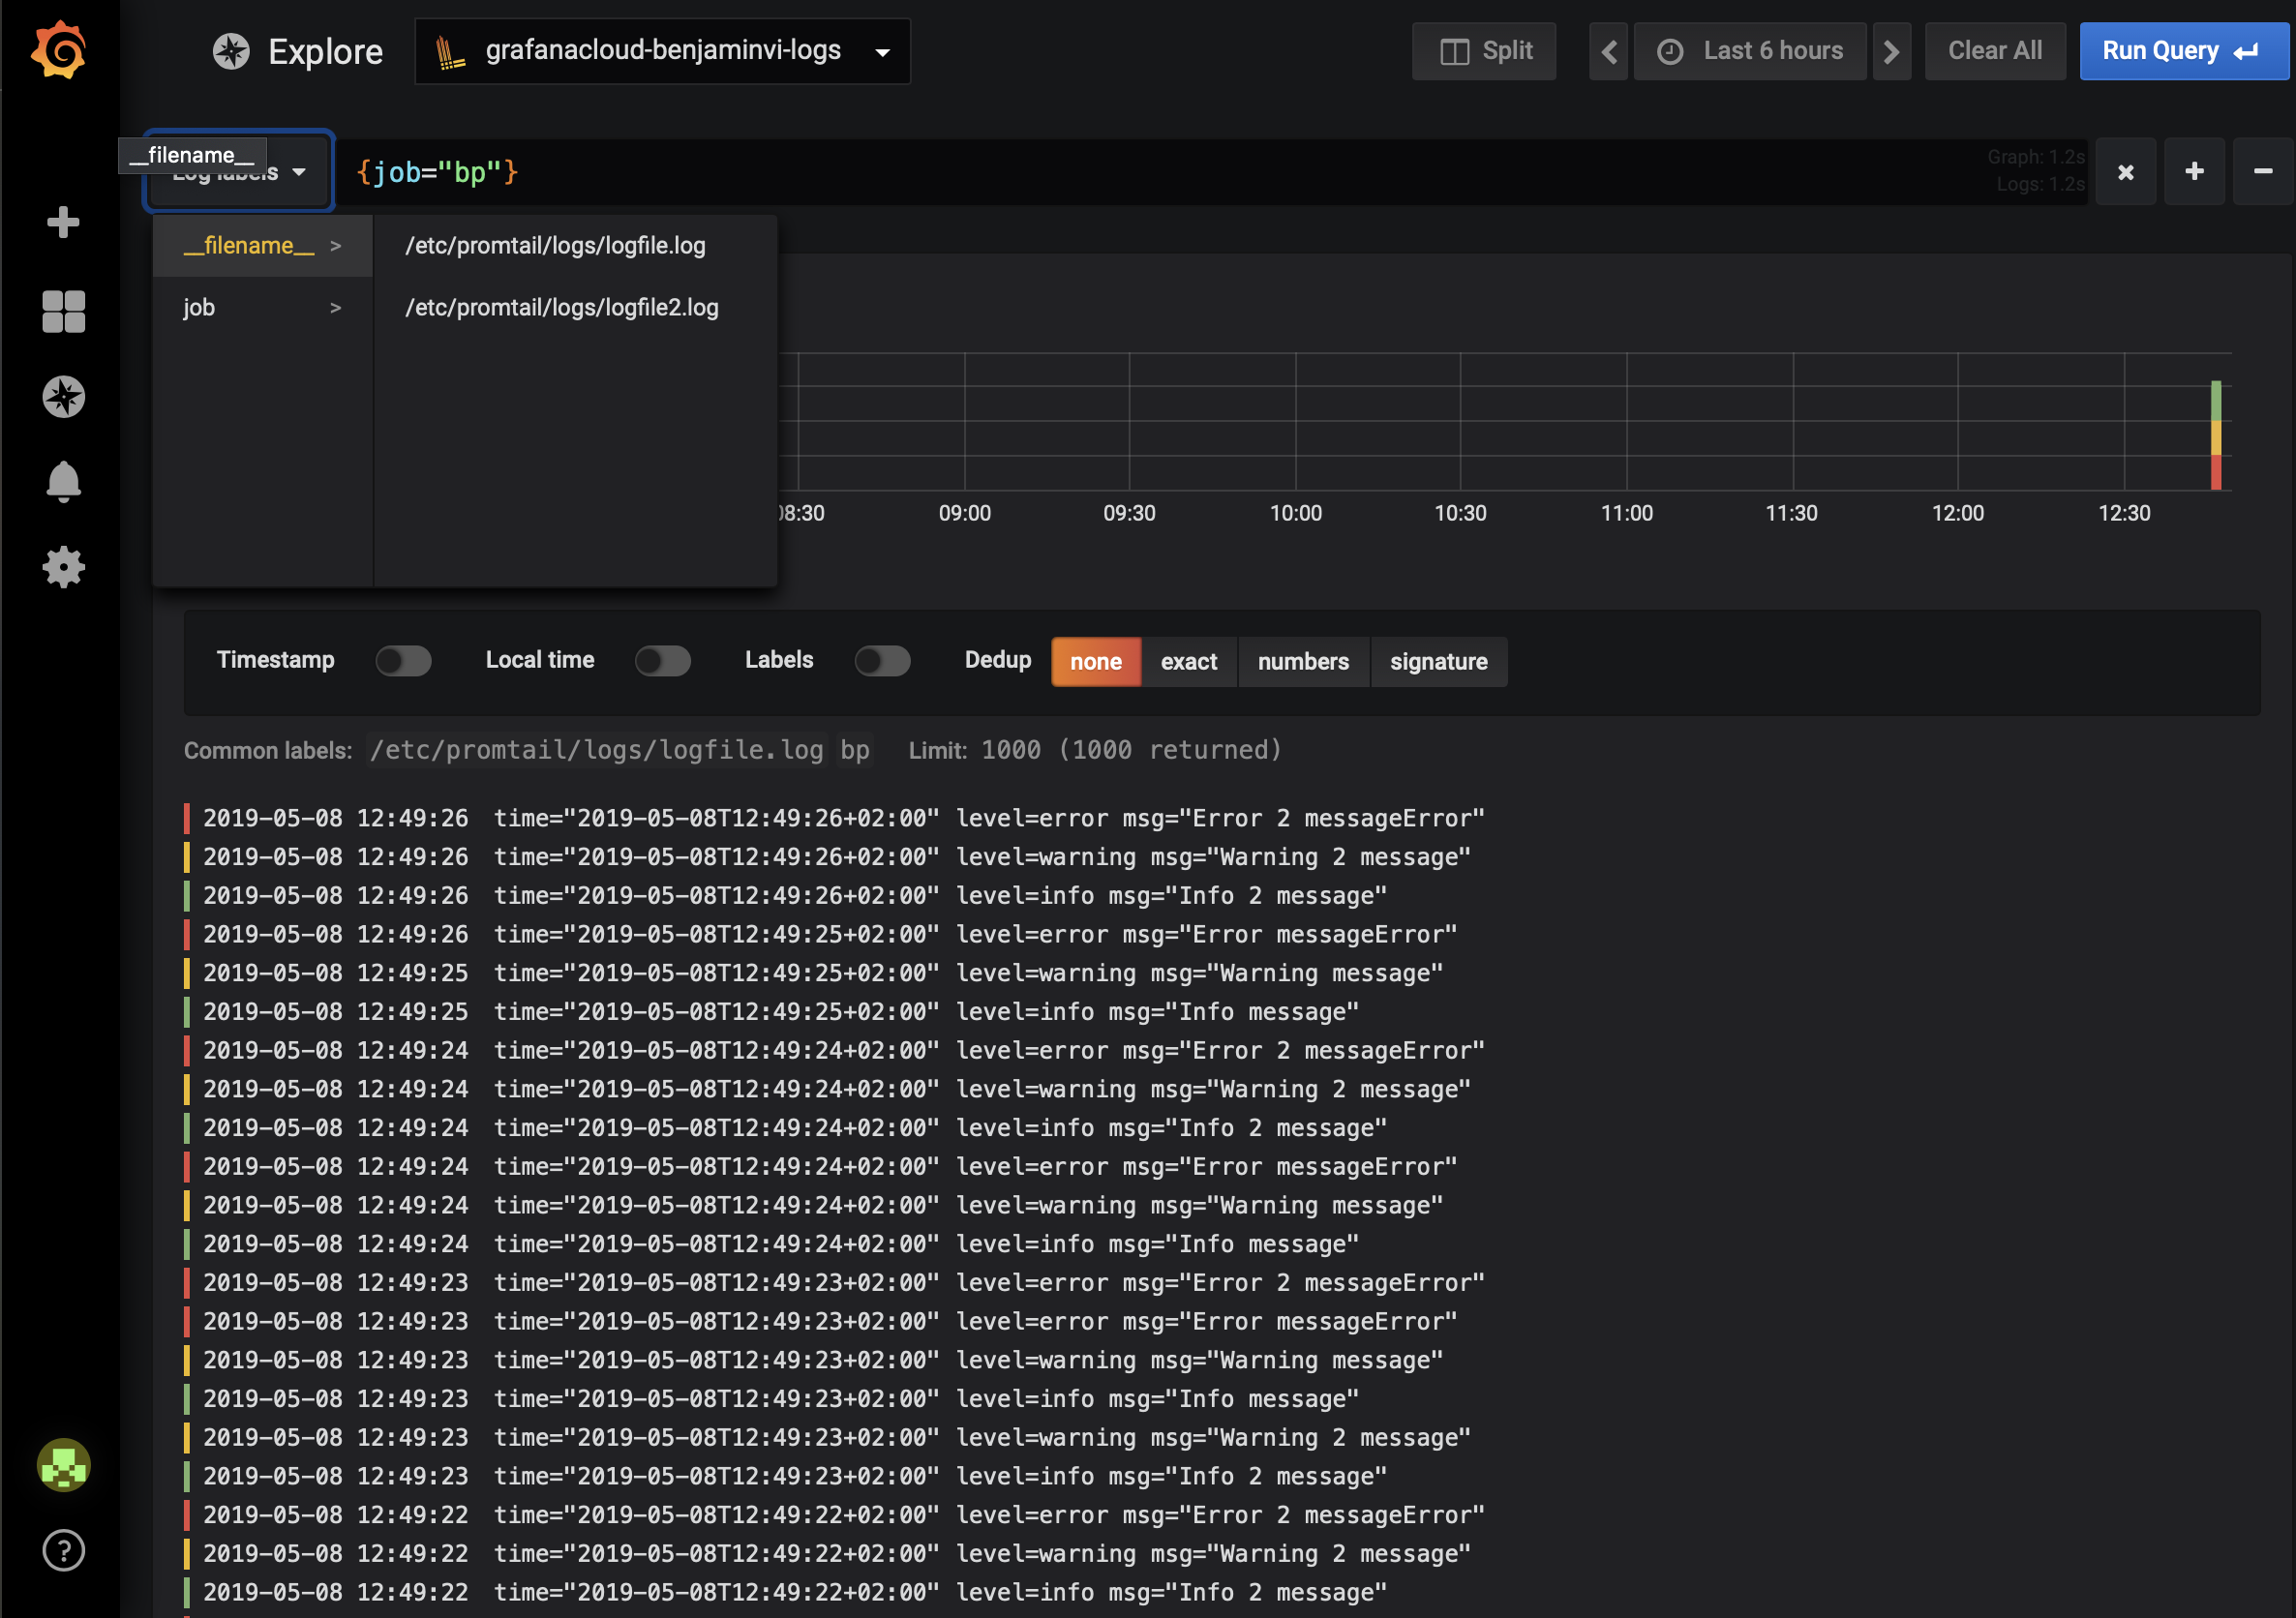
\includegraphics[scale=0.35]{img/loki_query}
    \caption[Loki query]{Loki query}
\end{figure}


\subsection{Kubernetes omgeving}

De Kubernetes deployment van deze oplossing is relatief eenvoudig. Grafana ondersteund nog geen dashboards en alerts voor een Loki datasource, daarom is het niet nodig om services hiervoor te deployen. Grafana kan simpelweg deployed worden op Kubernetes met de out-of-the-box docker image die te vinden is op de docker hub repository van Grafana. In Listing 7.7 wordt het commando hiervoor getoond. Om de Grafana UI te bereiken moet de Kubernetes poort hiervan nog geforward worden naar een eigen poort naar keuze. Dit gebeurt door gebruik te maken van het commando in Listing 7.8\\

\begin{lstlisting}[caption=Grafana Kubernetes deployment]
$kubectl create deployment grafana --image=docker.io/grafana/grafana:latest
\end{lstlisting}
\begin{lstlisting}[caption=Port-forwarding van Grafana]
$kubectl port-forward service/loki-grafana 3000:80
\end{lstlisting}

De andere componenten Promtail en Loki zijn te installeren via Helm charts die beschikbaar zijn in de github pagina van Grafana, namelijk github.com/grafana/loki/tree/master/production. Door gebrek aan documentatie valt hier geen extra uitleg bij te geven over de exacte configuratie die gebruikt wordt in deze Helm charts.


\section{Requirements}

\subsection{Must have}
\subsubsection{Moet open source zijn}
Voor elk van de onderzochte oplossingen geldt dezelfde score voor deze requirement, namelijk 5. Elk van de componenten waaruit een Loki `stack` bestaat, namelijk Promtail, Loki, en Grafana, is vrij te verkrijgen en te gebruiken.

\subsubsection{Ondersteuning voor cluster omgevingen zoals Kubernetes}
Loki is speciaal voor Kubernetes ontwikkeld. Deze oplossing kan ook buiten Kubernetes gebruikt worden maar werkt het best in een Kubernetes cluster. 

Om deze reden krijgt Loki een score van 5 op dit requirement.

\subsubsection{Moet een zo klein mogelijke impact hebben op de servers}
Loki heeft een minimale impact op de servers. Waar Elasticsearch gebruik maakt van volledige indexering bij het opslaan van logs, indexeert Loki enkel de metadata van logs waardoor het opslagverbruik lager ligt. Verder is ook nagedacht over de manier van het opslaan. De indexen worden opgeslagen in een object store. De logs worden via een distributor ondergebracht in ingestors. Deze worden gevuld met soortgelijke logs en worden opgeslagen in een NoSQL databank eens deze opgevuld zijn.

Om deze redenen krijgt Loki een score van 5 op dit requirement.

\subsubsection{Moet kunnen scalen naargelang de groeiende Kubernetes cluster}
Promtail, de log scraper van Loki, kan ook geconfigureerd worden als een DaemonSet waardoor automatische scaling gegarandeerd kan worden. 

Om deze reden krijgt Loki een score van 5 op dit requirement.

\subsection{Should have}
\subsubsection{Moet (relatief) eenvoudig te configureren zijn}
In het requirement `Moet goed gedocumenteerd zijn` hieronder zal nog verder uitgelegd worden waarom er weinig documentatie beschikbaar is. Het gebrek aan documentatie leidt tot een moeilijke configuratie voor een nieuwe gebruiker. Elk van de component zijn relatief eenvoudig te configureren eens wat meer ervaring is opgedaan.

Om deze redenen krijgt Loki een score van 3 op dit requirement.

\subsubsection{Moet (relatief) eenvoudig te gebruiken zijn}
Het gebruiksgemak van Loki wordt meteen duidelijk na de installatie en configuratie. Het overzicht van de logs en de manier waarop logs worden opgeslagen met labels  zorgen voor een aangename gebruikerservaring.

Om deze reden krijgt Loki een score van 5 op dit requirement.

\subsubsection{Moet goed gedocumenteerd zijn}
De documentatie van Loki is op het moment van schrijven quasi onbestaand. Buiten de officiële documentatie van Grafana zijn er slechts enkele bronnen beschikbaar. Dit is voornamelijk te wijten aan het feit dat Loki nog in een beta fase zit. Deze oplossing is nog niet zo lang geleden uitgekomen en wordt nog volop ontwikkeld. 

Om deze reden krijgt Loki een score van 2 op dit requirement.

\subsubsection{Moet de logs overzichtelijk kunnen tonen}
Grafana maakt gebruik van een eigen interface om de logs te tonen. Deze worden in een lijst van 1000 onder elkaar geplaatsd. Wanneer specifiek op zoek moet worden gegaan is er de mogelijk op te zoeken op labels en zo de getoonde lijst te verfijen. De query taal om logs te filteren is nog onder constructie waardoor de functionaliteit op dit moment vrij beperkt is. Dit is een belangrijke factor in de score van dit requirement

Om deze reden krijgt Loki een score van 2 op dit requirement.

\subsubsection{Ondersteuning voor verschillende plugins die data extra kunnen verwerken of naar meerdere locaties kunnen doorsturen}
Er zijn niet veel plugins beschikbaar die een soortgelijke functionaliteit hebben als beschreven in de requirement. Maar dit probleem is makkelijk op te lossen met het implementeren van Fluentd als log collector. Met deze configuratie scrapet Promtail al pod logs naar Fluentd. Deze verwerkt de logs en kan gebruik maken van een grote hoeveelheid plugins hiervoor. Na de verwerking worden de logs dan doorgestuurd naar Loki waar ze opgeslagen worden.

Om deze reden krijgt Loki een score van 4 op dit requirement.

\subsubsection{Ondersteuning voor visualisatie zoals grafieken}
Grafana heeft reeds ondersteuning voor grafieken en dergelijke voor het visualiseren van verschillende databronnen. Momenteel is Grafana ondersteuning voor een Loki databron aan het toevoegen voor dit onderdeel en zal ook aan deze requirement voldaan worden. Aangezien dit nog niet het geval is krijgt Loki een score van 1 voor deze requirement.

\subsection{Could have}
\subsubsection{Ondersteuning voor alerts}
Grafana heeft reeds ondersteuning voor alerts voor verschillende databronnen. Momenteel is Grafana ondersteuning voor een Loki databron aan het toevoegen voor dit onderdeel en zal ook aan deze requirement voldaan worden. Aangezien dit nog niet het geval is krijgt Loki een score van 1 voor deze requirement.

\section{Resultaten}
Zoals te zien is in tabel~\ref{tab:Loki-resultaten}, scoort Loki in eerste instantie niet zo hoog bij een standaard score op 5. Wanneer deze score wordt verwerkt aan de hand van belangrijkheidsgraad, is te zien dat Loki wel degelijk veel potentieel biedt. De score is gebaseerd op hoe Loki functioneert op het moment van schrijven van dit werk. Het product heeft nog een lange weg te gaan maar heeft reeds een perfecte score op de vier Must Have requirements. Mits wat verbeteringen op vlak van documentatie en visualisatie zal de score van Loki nog verbeteren.

Een uitgebreide conclusie is te vinden in Hoofdstuk~\ref{ch:conclusie} Conclusie.
\begin{table}[]
    \begin{tabular}{| m{20em} | m{2cm} | m{2cm} | m{2cm} | }
        \hline
        \textbf{Requirement}                                                                                              & \textbf{Score (op 5)} & \textbf{Multiplier} & \textbf{Score met multiplier} \\ \hline
        Moet open source zijn                                                                                             & 5                     & 10                  & 50                            \\ \hline
        Ondersteuning voor cluster omgevingen zoals Kubernetes                                                            & 5                     & 10                  & 50                            \\ \hline
        Moet een zo klein mogelijke impact hebben op de servers                                                           & 5                     & 10                  & 50                            \\ \hline
        Moet kunnen scalen naargelang de groeiende Kubernetes cluster                                                     & 5                     & 10                  & 50                            \\ \hline
        Moet (relatief) eenvoudig te configureren zijn                                                                    & 3                     & 5                   & 15                            \\ \hline
        Moet (relatief) eenvoudig te gebruiken zijn                                                                       & 5                     & 5                   & 25                            \\ \hline
        Moet goed gedocumenteerd zijn                                                                                     & 2                     & 5                   & 10                            \\ \hline
        Moet de logs overzichtelijk kunnen tonen                                                                          & 2                     & 5                   & 10                            \\ \hline
        Ondersteuning voor verschillende plugins die data extra kunnen verwerken of naar meerdere locaties kan doorsturen & 5                     & 5                   & 25                            \\ \hline
        Ondersteuning voor visualisatie zoals grafieken                                                                   & 1                     & 5                   & 5                             \\ \hline
        Ondersteuning voor alerts                                                                                         & 1                     & 1                   & 1                             \\ \hline
        \textbf{Totale score}                                                                                             & 39                    &                     & 291                           \\ \hline
    \end{tabular}
    \caption{Loki resultaten}
    \label{tab:Loki-resultaten}
\end{table}